\chapter{Tag 13 — Datenplatzierung im Datamatrix}

\begin{quote}
Aus Etappe 12 hast du zwölf Codewort-Bytes (5 Daten + 7 Prüfbytes)
für deinen HONIG-Code. Heute gehst du den schwierigsten algorithmischen
Schritt: \emph{wie kommt jedes Bit aus diesen zwölf Bytes an die
richtige Stelle im 12$\times$12-Modul-Raster?} Datamatrix nutzt dafür
ein Schema, das in der ISO-Spezifikation „ECC-200 placement" heißt —
und das wir heute Schritt für Schritt nachzeichnen.
\end{quote}

\section*{Lernziele für heute}

Am Ende von Tag 13 kannst du \dots

\begin{itemize}
\item erklären, warum Datamatrix die Codewords \emph{nicht} sequentiell
  von links oben nach rechts unten anordnet
\item die „Utah"-L-Form für ein einzelnes Codeword Bit für Bit ablesen
\item dem ECC-200-Cursor diagonal durchs Symbol folgen — und wissen,
  was an den vier Sonderecken passiert
\item das fertige Datenraster für deinen HONIG-Code erzeugen lassen
  und es mit der pylibdmtx-Referenz vergleichen
\end{itemize}

\paragraph{Material} Karopapier mit 12$\times$12-Raster, Bleistift,
Laptop mit Thonny und deinem RS-Encoder aus Etappe 12.

% =============================================================
\section{Warum nicht sequentiell? \normalfont(\textit{≈ 10 min})}
% =============================================================

Eine naive Idee: nimm die 96 Bits (12 Codewords à 8 Bit) und schreibe
sie zeilenweise von oben links nach unten rechts ins Datenraster.
Funktioniert technisch, ist aber didaktisch \emph{und} praktisch eine
Sackgasse.

\subsection*{Das Problem}

Wenn ein Kratzer eine kompakte Region des Symbols zerstört (z. B.
einen 3$\times$3-Block), wären \emph{alle} Bits eines bestimmten
Codeworts auf einen Schlag weg. Der Reed-Solomon-Decoder kann nur
$\lfloor t/2 \rfloor = 3$ Codeword-Fehler reparieren — bei sequenzieller
Anordnung wäre ein bisschen Schaden mehr als das Limit.

\subsection*{Die ECC-200-Lösung}

Datamatrix verteilt die acht Bits jedes Codeworts \emph{über das ganze
Symbol} — in einer L-förmigen „Utah"-Form. Ein lokaler Kratzer trifft
typischerweise je 1--2 Bits aus mehreren \emph{verschiedenen}
Codewords; der RS-Decoder verteilt die Last auf mehrere Korrektur-
Operationen, jede einzelne mit nur 1--2 Bit-Fehlern. Genau die Stelle,
für die er gut ist.

\section{Die „Utah"-L-Form für ein Codeword \normalfont(\textit{≈ 20 min})}

Jedes 8-Bit-Codeword wird als eine ganz bestimmte Anordnung von acht
Modulen ins Symbol gesetzt. Die acht Bits liegen in einer L-Form
relativ zu einem \emph{Cursor} (Zeile~$0$, Spalte~$0$):

\begin{center}
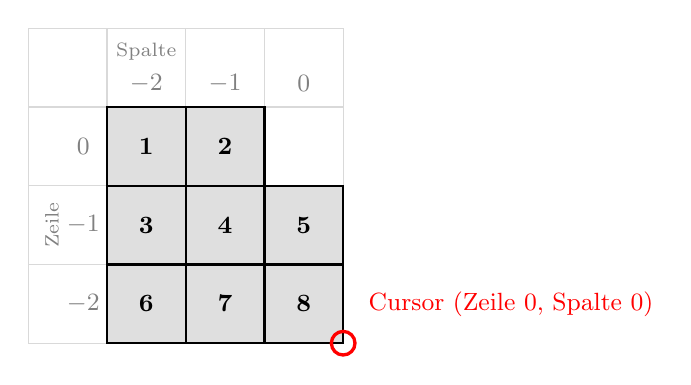
\begin{tikzpicture}[x=10mm, y=10mm, every node/.style={font=\small}]
  % Hintergrundraster 4×4 (col -3..0, row -3..0)
  \foreach \c in {-3,-2,-1,0,1}{
    \draw[gray!30, thin] (\c, -3) -- (\c, 1);
  }
  \foreach \r in {-3,-2,-1,0,1}{
    \draw[gray!30, thin] (-3, \r) -- (1, \r);
  }
  % Bit-Boxen (in Bildschirmkoordinaten: y nach oben = unsere -row)
  \fill[gray!25] (-2,-1) rectangle (-1,0); \node at (-1.5,-0.5) {\textbf{1}};
  \fill[gray!25] (-1,-1) rectangle (0,0);  \node at (-0.5,-0.5) {\textbf{2}};
  \fill[gray!25] (-2,-2) rectangle (-1,-1); \node at (-1.5,-1.5) {\textbf{3}};
  \fill[gray!25] (-1,-2) rectangle (0,-1);  \node at (-0.5,-1.5) {\textbf{4}};
  \fill[gray!25] (0,-2)  rectangle (1,-1);  \node at (0.5,-1.5)  {\textbf{5}};
  \fill[gray!25] (-2,-3) rectangle (-1,-2); \node at (-1.5,-2.5) {\textbf{6}};
  \fill[gray!25] (-1,-3) rectangle (0,-2);  \node at (-0.5,-2.5) {\textbf{7}};
  \fill[gray!25] (0,-3)  rectangle (1,-2);  \node at (0.5,-2.5)  {\textbf{8}};
  % Modul-Rahmen
  \draw[black, thick] (-2,-1) rectangle (-1,0);
  \draw[black, thick] (-1,-1) rectangle (0,0);
  \draw[black, thick] (-2,-2) rectangle (-1,-1);
  \draw[black, thick] (-1,-2) rectangle (0,-1);
  \draw[black, thick] (0,-2)  rectangle (1,-1);
  \draw[black, thick] (-2,-3) rectangle (-1,-2);
  \draw[black, thick] (-1,-3) rectangle (0,-2);
  \draw[black, thick] (0,-3)  rectangle (1,-2);
  % Cursor-Markierung
  \draw[red, very thick] (1,-3) circle (0.15);
  \node[red, anchor=west] at (1.2,-2.5) {Cursor (Zeile 0, Spalte 0)};
  % Achsenbeschriftung
  \foreach \c/\lab in {-2/{$-2$}, -1/{$-1$}, 0/{$0$}}{
    \node[gray] at (\c+0.5, 0.3) {\lab};
  }
  \foreach \r/\lab in {-2/{$-2$}, -1/{$-1$}, 0/{$0$}}{
    \node[gray] at (-2.3, \r-0.5) {\lab};
  }
  \node[gray, font=\scriptsize] at (-1.5, 0.7) {Spalte};
  \node[gray, font=\scriptsize, rotate=90] at (-2.7, -1.5) {Zeile};
\end{tikzpicture}
\end{center}

Drei Module oben links, drei Module diagonal in der Mitte, zwei
unten. Bit 1 ist das höchstwertige (MSB, Wert 128), Bit 8 das
niedrigstwertige (LSB, Wert 1).

\paragraph{Warum „Utah"?}
Schau dir den US-Bundesstaat \textbf{Utah} mal auf einer Landkarte
an (oder auf Wikipedia). Sein Umriss hat eine charakteristische
L-Form — ein großes Rechteck mit einer rechteckigen Ecke oben rechts
herausgeschnitten. Genau das macht auch unsere Bit-Anordnung: ein
„volles" 3$\times$3-Quadrat, dem oben rechts ein Modul fehlt. Die
Datamatrix-Erfinder haben sich diese Eselsbrücke ausgedacht — und der
Name ist in Spec und Implementierungen geblieben (du findest in
Open-Source-Encodern oft Funktionen, die einfach
\texttt{place\_utah} heißen, ohne weitere Erklärung).

\paragraph{Hilfe: Dezimal $\to$ Binär in 8 Bit}
Bevor du eine Codewort-Zahl in die Utah-Form einträgst, brauchst du
ihre 8 Bits. Hier die \emph{Stellenwert-Tabelle} für ein Byte:

\begin{center}
\small
\begin{tabular}{c | c c c c c c c c}
\toprule
\textbf{Bit-Nr.} & 1 & 2 & 3 & 4 & 5 & 6 & 7 & 8 \\
\textbf{Stellenwert} & 128 & 64 & 32 & 16 & 8 & 4 & 2 & 1 \\
\midrule
\textbf{Beispiel 73} & 0 & 1 & 0 & 0 & 1 & 0 & 0 & 1 \\
\bottomrule
\end{tabular}
\end{center}

Faustregel zum Umrechnen: nimm die Zahl und gehe die Stellenwerte
von links nach rechts (128, 64, 32, \dots, 1) durch. Bei jedem
Stellenwert: passt er noch in die Restzahl? Wenn ja: Bit \texttt{1},
Stellenwert abziehen. Wenn nein: Bit \texttt{0}, weitergehen.

Konkret für $73$:

\begin{itemize}
\item $128 > 73$? ja $\to$ Bit 1 = \texttt{0}
\item $64 \le 73$? ja $\to$ Bit 2 = \texttt{1}, Restzahl: $73 - 64 = 9$
\item $32 > 9$? ja $\to$ Bit 3 = \texttt{0}
\item $16 > 9$? ja $\to$ Bit 4 = \texttt{0}
\item $8 \le 9$? ja $\to$ Bit 5 = \texttt{1}, Rest: $9 - 8 = 1$
\item $4 > 1$? ja $\to$ Bit 6 = \texttt{0}
\item $2 > 1$? ja $\to$ Bit 7 = \texttt{0}
\item $1 \le 1$? ja $\to$ Bit 8 = \texttt{1}, Rest $0$ \checkmark
\end{itemize}

Ergebnis: $73_{10} = \texttt{01001001}_2 = 64 + 8 + 1$. Probe geht
auf — die Stellenwerte aller \texttt{1}-Bits aufsummiert ergeben
wieder die Ausgangszahl.

\paragraph{Bit-Tabelle für alle 12 HONIG-Codewörter}
Damit du die Umrechnung nicht für jedes Codeword einzeln machen
musst — hier die komplette Tabelle für unseren Honig-Code
\texttt{[73, 80, 79, 74, 72, 70, 186, 97, 167, 44, 40, 243]}:

\begin{center}
\small
\begin{tabular}{c c | c c c c c c c c}
\toprule
\textbf{Nr.} & \textbf{Wert} & \textbf{Bit 1} & \textbf{2} & \textbf{3} & \textbf{4} & \textbf{5} & \textbf{6} & \textbf{7} & \textbf{Bit 8} \\
                &           & (128) & (64) & (32) & (16) & (8) & (4) & (2) & (1) \\
\midrule
\phantom{0}1  &  73 & 0 & 1 & 0 & 0 & 1 & 0 & 0 & 1 \\
\phantom{0}2  &  80 & 0 & 1 & 0 & 1 & 0 & 0 & 0 & 0 \\
\phantom{0}3  &  79 & 0 & 1 & 0 & 0 & 1 & 1 & 1 & 1 \\
\phantom{0}4  &  74 & 0 & 1 & 0 & 0 & 1 & 0 & 1 & 0 \\
\phantom{0}5  &  72 & 0 & 1 & 0 & 0 & 1 & 0 & 0 & 0 \\
\phantom{0}6  &  70 & 0 & 1 & 0 & 0 & 0 & 1 & 1 & 0 \\
\phantom{0}7  & 186 & 1 & 0 & 1 & 1 & 1 & 0 & 1 & 0 \\
\phantom{0}8  &  97 & 0 & 1 & 1 & 0 & 0 & 0 & 0 & 1 \\
\phantom{0}9  & 167 & 1 & 0 & 1 & 0 & 0 & 1 & 1 & 1 \\
10            &  44 & 0 & 0 & 1 & 0 & 1 & 1 & 0 & 0 \\
11            &  40 & 0 & 0 & 1 & 0 & 1 & 0 & 0 & 0 \\
12            & 243 & 1 & 1 & 1 & 1 & 0 & 0 & 1 & 1 \\
\bottomrule
\end{tabular}
\end{center}

Bit 1 ist das MSB (Wert $128$), Bit 8 das LSB (Wert $1$). Wenn du
GRETA oder ein anderes Wort zeichnest, baust du dir die gleiche
Tabelle für deine 12 Codewörter aus Etappe 12 — der Lösungsanhang
zeigt das Beispiel für GRETA.

\begin{bleistiftuebung}{1}{Utah-Form für ein Beispiel-Codeword}
Nimm das HONIG-Codeword Nummer 1: das ist \texttt{73} (Bit-Muster
\texttt{01001001}). Trage die acht Bits in die Utah-Form ein:

\begin{itemize}
\item Bit 1 (MSB) = $0$, Bit 2 = $1$
\item Bit 3 = $0$, Bit 4 = $0$, Bit 5 = $1$
\item Bit 6 = $0$, Bit 7 = $0$, Bit 8 (LSB) = $1$
\end{itemize}

Wenn der Cursor bei (\texttt{row}, \texttt{col}) = (4, 0) steht (das
ist die Startposition im ECC-200-Algorithmus), liegen die acht
Bits in den Modul-Positionen (2,$-2$), (2,$-1$), (3,$-2$), (3,$-1$),
(3,0), (4,$-2$), (4,$-1$), (4,0). Negative Spalten? Da kommt der
\emph{Wrap-around}-Mechanismus ins Spiel.
\end{bleistiftuebung}

\subsection*{Wrap-around am Symbol-Rand}

Wenn die Utah-Form über den Rand des Symbols hinausragt, wickelt sie
sich auf der gegenüberliegenden Seite ein — genau wie das Geschenkpapier
um einen Karton:

\begin{center}
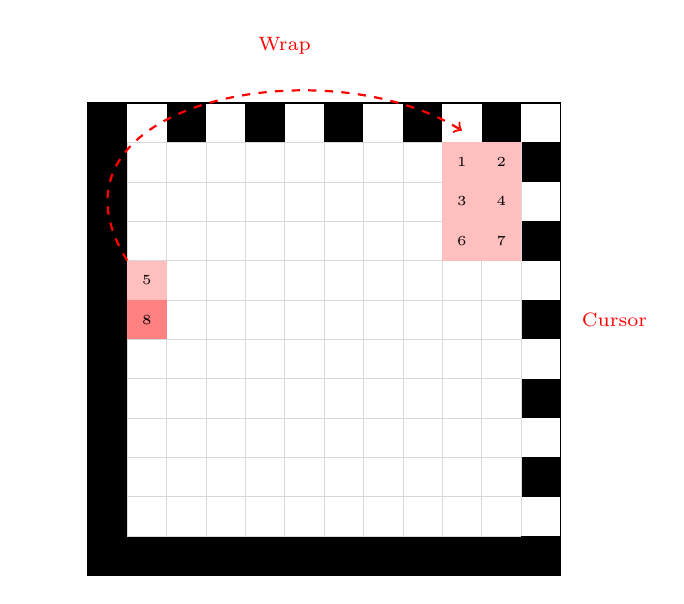
\begin{tikzpicture}[x=5mm, y=-5mm, every node/.style={font=\tiny}]
  % L-Pattern unten (Datamatrix-Zeile 11)
  \foreach \c in {0,...,11}{ \fill[black] (\c, 11) rectangle (\c+1, 12); }
  % L-Pattern links (Spalte 0)
  \foreach \r in {0,...,10}{ \fill[black] (0, \r) rectangle (1, \r+1); }
  % Zeitsignal oben (Zeile 0): an geraden Spalten schwarz
  \foreach \c in {0, 2, 4, 6, 8, 10}{ \fill[black] (\c, 0) rectangle (\c+1, 1); }
  % Zeitsignal rechts (Spalte 11): an ungeraden Zeilen schwarz
  \foreach \r in {1, 3, 5, 7, 9}{ \fill[black] (11, \r) rectangle (12, \r+1); }
  % Hilfsraster im Innenbereich
  \foreach \i in {1,...,11}{
    \draw[gray!30, very thin] (\i, 1) -- (\i, 11);
    \draw[gray!30, very thin] (1, \i) -- (11, \i);
  }
  % Symbol-Aussenrahmen
  \draw[black] (0, 0) rectangle (12, 12);
  % Bit 5 (innen): inner (3, 0) → Symbol (4, 1)
  \fill[red!25] (1, 4) rectangle (2, 5); \node at (1.5, 4.5) {5};
  % Bit 8 (Cursor-Position): inner (4, 0) → Symbol (5, 1)
  \fill[red!50] (1, 5) rectangle (2, 6); \node at (1.5, 5.5) {8};
  % Wrap-Bits 1..4, 6, 7: rechts oben im Symbol
  \fill[red!25] (9, 1) rectangle (10, 2);  \node at (9.5, 1.5)  {1};
  \fill[red!25] (10, 1) rectangle (11, 2); \node at (10.5, 1.5) {2};
  \fill[red!25] (9, 2) rectangle (10, 3);  \node at (9.5, 2.5)  {3};
  \fill[red!25] (10, 2) rectangle (11, 3); \node at (10.5, 2.5) {4};
  \fill[red!25] (9, 3) rectangle (10, 4);  \node at (9.5, 3.5)  {6};
  \fill[red!25] (10, 3) rectangle (11, 4); \node at (10.5, 3.5) {7};
  % Wrap-Pfeil
  \draw[red, dashed, thick, ->] (1.0, 4.0) .. controls (-1.5, 0) and (6, -1.5) .. (9.5, 0.7);
  \node[red, anchor=south, font=\scriptsize] at (5, -1.0) {Wrap};
  \node[red, anchor=west, font=\scriptsize] at (12.3, 5.5) {Cursor};
\end{tikzpicture}
\end{center}

Cursor steht bei \texttt{(Zeile 4, Spalte 0)}. Bit 5 und Bit 8 (im
Bild rot) liegen \emph{innerhalb} des Symbols. Die anderen sechs Bits
würden über den linken Rand hinaus rutschen — und tauchen
stattdessen oben rechts wieder auf, leicht versetzt. Genau das
beschreibt die Wrap-Formel:

\begin{itemize}
\item Wenn \texttt{row < 0}: nimm \texttt{row + n} und verschiebe
  \texttt{col} um $4 - ((n+4) \bmod 8)$.
\item Wenn \texttt{col < 0}: analog mit \texttt{col + n}.
\end{itemize}

Klingt wild, garantiert aber: jedes Datenmodul wird genau einmal
belegt, und das ohne Lücken.

\begin{pythoneinheit}{1}{Utah-Form als Code}
\pythoncodeteil{tag13/placement.py}{utah}

\texttt{\_place\_one} setzt einen einzelnen Bit-Slot mit der Wrap-
Logik; \texttt{\_place\_utah} ruft das achtmal mit den passenden
Offsets auf. Wir setzen hier nicht die Bits direkt ein, sondern
markieren das Layout-Raster mit Tupeln \texttt{(codeword\_nr, bit\_nr)}
— dazu gleich mehr beim Hauptalgorithmus.
\end{pythoneinheit}

% =============================================================
\section{Die vier Sonderecken \normalfont(\textit{≈ 15 min})}
% =============================================================

In den vier Symbolecken passt die Standard-Utah-Form aus geometrischen
Gründen nicht — die Wrap-Bewegung würde dort Lücken oder
Doppelbelegungen erzeugen. Der Standard löst das mit \emph{vier
Sonder-Patterns} (Corner1 bis Corner4), die jeweils ein einzelnes
Codeword mit acht Modulen anders verteilt platzieren.

Welcher Corner wann zuschlägt, hängt von der Symbol-Größe ab:

\begin{itemize}
\item \textbf{Corner 1} an der unteren-linken/oberen-rechten Ecke
  (immer)
\item \textbf{Corner 2} bei Symbolgrößen mit $n \bmod 4 \ne 0$
\item \textbf{Corner 3} bei $n \bmod 8 = 4$ (gilt für 12$\times$12!)
\item \textbf{Corner 4} bei $n \bmod 8 = 0$
\end{itemize}

Für unser 12$\times$12-Symbol sind also Corner 1 und Corner 3 aktiv.

\begin{pythoneinheit}{2}{Die vier Eckpatterns}
\pythoncodeteil{tag13/placement.py}{corners}

Vier kleine Funktionen — jede fest verdrahtet für die spezifische
Modul-Verteilung an ihrer Ecke. Klingt willkürlich, ist aber präzise
in ISO/IEC 16022 Annex F spezifiziert; die Form ist Konvention, wie
das Modulo-Polynom aus Etappe 12.
\end{pythoneinheit}

% =============================================================
\section{Der Hauptalgorithmus — Cursor diagonal durchs Symbol \normalfont(\textit{≈ 25 min})}
% =============================================================

Der Cursor startet bei (\texttt{row}, \texttt{col}) = (4, 0) — also
vier Zeilen unter dem oberen Rand, ganz links. Dann wechselt er
zwischen zwei Diagonal-Richtungen:

\begin{center}
\begin{tikzpicture}[x=5mm, y=-5mm, every node/.style={font=\tiny}]
  % L-Pattern unten (Datamatrix-Zeile 11)
  \foreach \c in {0,...,11}{ \fill[black] (\c, 11) rectangle (\c+1, 12); }
  % L-Pattern links (Spalte 0)
  \foreach \r in {0,...,10}{ \fill[black] (0, \r) rectangle (1, \r+1); }
  % Zeitsignal oben (Zeile 0)
  \foreach \c in {0, 2, 4, 6, 8, 10}{ \fill[black] (\c, 0) rectangle (\c+1, 1); }
  % Zeitsignal rechts (Spalte 11)
  \foreach \r in {1, 3, 5, 7, 9}{ \fill[black] (11, \r) rectangle (12, \r+1); }
  % Hilfsraster im Innenbereich
  \foreach \i in {1,...,11}{
    \draw[gray!25, very thin] (\i, 1) -- (\i, 11);
    \draw[gray!25, very thin] (1, \i) -- (11, \i);
  }
  % Symbol-Aussenrahmen
  \draw[black] (0, 0) rectangle (12, 12);
  % Pfade in Symbol-Koordinaten (Datamatrix Zeile/Spalte; y-Achse zeigt nach unten):
  % Start (4, 0) inner == (5, 1) Symbol; Mitte des Moduls bei (1.5, 5.5)
  % Sweep 1 (hoch-rechts): inner (4,0)→(2,2)→(0,4)  ⇒ Symbol (5,1)→(3,3)→(1,5)
  \draw[blue, thick, ->] (1.5, 5.5) -- (3.5, 3.5);
  \draw[blue, thick, ->] (3.5, 3.5) -- (5.5, 1.5);
  % Versatz: row += 1, col += 3  ⇒ inner (1, 3) ⇒ Symbol (2, 4)
  \draw[gray!70, dashed] (5.5, 1.5) -- (4.5, 2.5);
  % Sweep 2 (runter-links): inner (1,3)→(3,1)  ⇒ Symbol (2,4)→(4,2)
  \draw[teal, thick, ->] (4.5, 2.5) -- (2.5, 4.5);
  % Versatz: row += 3, col += 1  ⇒ inner (6, 2) ⇒ Symbol (7, 3)
  \draw[gray!70, dashed] (2.5, 4.5) -- (3.5, 7.5);
  % Sweep 3 (hoch-rechts): inner (6,2)→(4,4)→(2,6)→(0,8)
  \draw[blue, thick, ->] (3.5, 7.5) -- (5.5, 5.5);
  \draw[blue, thick, ->] (5.5, 5.5) -- (7.5, 3.5);
  \draw[blue, thick, ->] (7.5, 3.5) -- (9.5, 1.5);
  % Versatz: inner (1, 7) ⇒ Symbol (2, 8)
  \draw[gray!70, dashed] (9.5, 1.5) -- (8.5, 2.5);
  % Sweep 4 (runter-links): inner (1,7)→(3,5)→(5,3)→(7,1)
  \draw[teal, thick, ->] (8.5, 2.5) -- (6.5, 4.5);
  \draw[teal, thick, ->] (6.5, 4.5) -- (4.5, 6.5);
  \draw[teal, thick, ->] (4.5, 6.5) -- (2.5, 8.5);
  % Cursor-Marker
  \draw[red, very thick] (1.5, 5.5) circle (0.25);
  \node[red, anchor=east, font=\scriptsize] at (-0.3, 5.5) {Start};
  % Legende
  \node[blue, anchor=west, font=\scriptsize] at (12.3, 2.5) {Sweep ↗};
  \node[teal, anchor=west, font=\scriptsize] at (12.3, 4.5) {Sweep ↙};
  \node[gray!70, anchor=west, font=\scriptsize] at (12.3, 6.5) {Versatz};
\end{tikzpicture}
\end{center}

\begin{itemize}
\item \textbf{Hoch-rechts (blau)}: pro Schritt zwei Zeilen nach oben
  und zwei Spalten nach rechts ($\Delta\text{row} = -2$, $\Delta\text{col}
  = +2$). An jeder Position eine Utah-Form setzen, falls noch frei.
\item \textbf{Runter-links (türkis)}: umgekehrt — zwei Zeilen runter,
  zwei Spalten links ($\Delta\text{row} = +2$, $\Delta\text{col} = -2$).
\end{itemize}

Zwischen den Richtungswechseln versetzt der Cursor sich um
(\texttt{+1 row, +3 col}) bzw. (\texttt{+3 row, +1 col}) (im
Diagramm gestrichelte graue Linien) — sodass er beim nächsten
Diagonal-Sweep eine neue Utah-Reihe abdeckt.

\subsection*{Erst Layout, dann Bits}

Wir bauen zuerst das \emph{Layout} — eine Matrix, die für jedes Modul
nur sagt: „hier kommt Bit \texttt{n} von Codeword \texttt{c} hin",
ohne den konkreten Wert. Erst danach setzen wir die echten Bits aus
unseren Codewords ein.

Vorteil: das Layout ist für \emph{jedes} 12$\times$12-Symbol gleich
(die Geometrie hängt nicht vom Inhalt ab). Wir können das Layout-
Raster ein Mal berechnen und dann beliebig viele Codewort-Folgen
hineinprojizieren.

\begin{pythoneinheit}{3}{Hauptalgorithmus und Codewort-Projektion}
\pythoncodeteil{tag13/placement.py}{main}

\texttt{\_build\_layout} läuft den Cursor durchs Symbol und markiert
jedes Datenmodul mit (codeword, bit). \texttt{place\_codewords}
projiziert dann die echten Bits aus der Codeword-Liste in eine
12$\times$12-Matrix und füllt die vier ungenutzten „Padding-Slots"
unten rechts mit dem festgelegten Schachbrett-Muster (das ist eine
Datamatrix-Eigenheit für 12$\times$12 — bei größeren Symbolen sind
alle Slots belegt).

Wichtige Konvention: das Layout wird auf einer 10$\times$10-
\emph{Innenfläche} gebaut, weil L-Pattern und Zeitsignal die äußeren
12$\times$12-Ränder belegen. Die Projektion verschiebt den Innen-Index
$(r, c)$ auf den Symbol-Index $(r+1, c+1)$.
\end{pythoneinheit}

\begin{pythoneinheit}{4}{Demo: Datenbereich für HONIG erzeugen}
\pythoncodeteil{tag13/placement.py}{demo}

Wenn du \texttt{verify\_against\_reference()} ausführst, baut Python
für HONIG (und GRETA) das Datenraster und vergleicht es Modul für
Modul mit dem, was die Bibliothek pylibdmtx aus demselben Text
erzeugt. Bei \texttt{✓ HONIG matches} weißt du: dein eigener Encoder
produziert exakt die gleichen Module wie ein produktiv eingesetzter
Datamatrix-Encoder. Das ist der Beweis, dass der Algorithmus korrekt
ist — ohne Bibliothek im Encoding-Pfad.
\end{pythoneinheit}

% =============================================================
\section{Hand-Werkstattbogen \normalfont(\textit{≈ 50 min})}
% =============================================================

Genug Theorie — jetzt zeichnest du. Die Datei
\texttt{zeichenvorlage-datamatrix.pdf} liegt diesem Buch bei (zwei
A4-Seiten: ein vorgemachtes HONIG-Symbol und ein leeres Feld für
deinen eigenen Code).

Auf jedem Blatt findest du:

\begin{itemize}
\item ein \textbf{12$\times$12-Modul-Raster} mit dem L-Pattern (untere
  und linke Kante schwarz) und dem Zeitsignal (obere und rechte Kante
  abwechselnd) bereits vorgezeichnet
\item eine \textbf{Hilfstabelle} mit zwölf Zeilen — eine pro Codeword
  — zum Eintragen von Wert (dezimal), 8-Bit-Pattern und der Position
  jedes Bits im Symbol
\item Platz, um deine Berechnung aus Etappe 12 (Codewort-Bytes inkl.
  ECC) einzutragen
\end{itemize}

\begin{bleistiftuebung}{2}{HONIG zeichnen}
Trage in das Vorbild-Feld die HONIG-Codewort-Bytes
\texttt{[73, 80, 79, 74, 72, 70, 186, 97, 167, 44, 40, 243]}
in die Hilfstabelle ein. Schwarze Module der Reihe nach
ausfüllen. Das Vorbild zeigt dir das Ergebnis bereits — vergleiche
beim Zeichnen.
\end{bleistiftuebung}

\begin{bleistiftuebung}{3}{Eigenes Symbol zeichnen}
Auf dem zweiten Blatt: trage deine eigenen Codewort-Bytes ein
(GRETA aus Etappe 12 oder ein eigenes 5-Buchstaben-Wort, dessen
ECC du selbst berechnet hast). Zeichne das Datenraster Modul für
Modul. \emph{Nicht} die Geduld verlieren — selbst routinierte
Datamatrix-Forscher brauchen für ein 12$\times$12-Symbol von Hand
30--45 Minuten beim ersten Mal. Auf dem zweiten Blatt sind die
Module bereits in der Codeword-Farbe markiert und mit „c/b"
beschriftet (Codeword-Nummer und Bit-Nummer), damit du
sofort weißt, welches Modul zu welchem Byte gehört.
\end{bleistiftuebung}

% --- Werkstatt-Bogen als integriertes Beilage-PDF ---
% pdf/zeichenvorlage-datamatrix.pdf wird vor dem Hauptbuch/Auszug
% gebaut (siehe Makefile-Abhängigkeit). Zwei A4-Seiten hochkant:
% Seite 1 mit dem fertig gezeichneten HONIG-Vorbild, Seite 2 mit
% dem farbig vorcodierten leeren Feld zum Selber-Zeichnen.
\includepdf[pages=-]{../pdf/zeichenvorlage-datamatrix.pdf}

% =============================================================
\section{Reflexion und Brücke zu Tag 14 \normalfont(\textit{≈ 10 min})}
% =============================================================

Du hast jetzt:

\begin{itemize}
\item den ECC-200-Datenplatzierungs-Algorithmus verstanden — Utah-Form,
  diagonale Cursor-Bewegung, vier Sonderecken
\item eine Python-Implementation, die exakt mit pylibdmtx übereinstimmt
\item ein vollständig handgezeichnetes 12$\times$12-Datamatrix-Symbol mit
  deinem eigenen Wort
\end{itemize}

Was noch fehlt für den Scan-Test:

\begin{itemize}
\item L-Pattern und Zeitsignal sind in der Werkstattbogen-Vorlage
  schon vorgezeichnet, aber bei einem komplett selbstgemachten Symbol
  (auf leerem Karopapier) müssten sie auch entstehen — Tag 14.
\item Der Scan-Test mit dem Handy — auch Tag 14.
\item Ein Vergleich Hand-Symbol vs. Python-Symbol (PNG ausgedruckt) —
  zur Selbstkontrolle.
\end{itemize}

\subsection*{Vorschau Tag 14}

Wir setzen das L-Pattern und Zeitsignal um deinen Datenbereich, sodass
ein vollständiges, scannbares Symbol entsteht. Plus: einen Mini-Encoder
in 60 Zeilen Python, der aus einem Wort das fertige PNG produziert —
ohne irgendeine Drittbibliothek im Encoding-Pfad. Und der finale
Beweis: dein selbstgezeichneter Honig-Datamatrix wird vom Handy
gelesen und sagt \texttt{HONIG}.
